\documentclass[14pt]{beamer}
\usetheme{Warsaw}
\usepackage[utf8]{vietnam}
\usepackage{ragged2e}
\usepackage{framed}
\useoutertheme{shadow}
%\setbeamertemplate{navigation symbols}{}
\setbeamertemplate{frametitle}[default][center]
\setbeamertemplate{headline}
{
  \leavevmode%
  \hbox{%
  \begin{beamercolorbox}[wd=.5\paperwidth,ht=2.65ex,dp=1.5ex,right]{section in head/foot}%
    \usebeamerfont{section in head/foot}\insertsectionhead\hspace*{2ex}
  \end{beamercolorbox}%
  \begin{beamercolorbox}[wd=.5\paperwidth,ht=2.65ex,dp=1.5ex,left]{subsection in head/foot}%
    \usebeamerfont{subsection in head/foot}\hspace*{2ex}\insertsubsectionhead
  \end{beamercolorbox}}%
  \vskip0pt%
}

\newcommand*\oldmacro{}
\let\oldmacro\insertshortauthor
\renewcommand*\insertshortauthor{
      \leftskip=.3cm
      \insertframenumber\,/\,\inserttotalframenumber\hfill\oldmacro
}

\usepackage{graphicx}
\usepackage{hyperref}
\hypersetup{
  colorlinks        = false,
  bookmarksnumbered = true,
  unicode           = true,
  pdfauthor         = {Duong Tien Thuan - 50TH2 - 0851061294},
  pdftitle          = {TIEP CAN SYSTEM AUTOMATION CHO HA TANG SAN PHAM CONG NGHE},
  pdfsubject        = {DO AN TOT NGHIEP - CSE - WRU},
  pdfcreator        = {Thuan Duong <thuandt26@gmail.com>},
  pdfproducer       = {pdflatex}
}

\title[Tiếp cận System Automation cho hạ tầng sản phẩm công nghệ]{Tiếp cận System Automation cho hạ tầng sản phẩm công nghệ}
\author[Dương Tiến Thuận - 50TH2]{SV: Dương Tiến Thuận - 50TH2\\GVHD: Th.S Nguyễn Nam Hưng}

\begin{document}

\AtBeginSection[]
{
  \begin{frame}
    \frametitle{Nội dung}
    \tableofcontents[currentsection]
  \end{frame}
}

\AtBeginSubsection[]
{
  \begin{frame}
    \frametitle{Nội dung}
    \tableofcontents[currentsection,currentsubsection]
  \end{frame}
}

\begin{frame}{BẢO VỆ ĐỒ ÁN TỐT NGHIỆP}
    \titlepage
\end{frame}

  \begin{frame}
    \frametitle{Nội dung}
    \tableofcontents
  \end{frame}

\section{Tổng quan}
\subsection*{Lý do cần sự tự động hóa}
\begin{frame}{Lý do cần sự tự động hóa}
  \begin{alertblock}\justifying
    \Large Giảm thiểu sự nhàm chán và tăng hiệu quả công việc khi phải thực hiện hàng loạt những công việc lặp đi lặp lại nhiều lần.
  \end{alertblock}
\end{frame}

\subsection*{Các vấn đề nảy sinh}

\begin{frame}{Các vấn đề nảy sinh}
\renewcommand{\baselinestretch}{1.50}\normalsize
  \begin{itemize}
    \item \large Vấn đề của con người: Quên và Nhớ !?
    \item \large Hệ thống biến thành một "vũng lầy".
  \end{itemize}
\renewcommand{\baselinestretch}{1.0}\normalsize
\end{frame}

\subsection{Cách giải quyết vấn đề}

\begin{frame}{Cách giải quyết vấn đề}
\renewcommand{\baselinestretch}{1.50}\normalsize
  \begin{itemize}
    \item \Large Chuẩn hóa quy trình làm việc.
    \pause
    \item \Large Chấp nhận sống với "vũng lầy".
    \pause
    \item \Large Tự động hóa hệ thống.
  \end{itemize}
\renewcommand{\baselinestretch}{1.0}\normalsize
\end{frame}

\subsection{Sự cần thiết của các công cụ tự động hóa}
\begin{frame}{Sự cần thiết của các công cụ tự động hóa}
  \begin{itemize}
    \item Các kịch bản tùy chỉnh thường phức tạp và không có tài liệu kèm theo.
    \pause
    \item Các kịch bản tùy chỉnh ít có khả năng mở rộng hoặc sử dụng lại.
    \pause
    \item Sự gia tăng số lượng máy chủ phải quản lý do sự phát triển của công nghệ điện toán đám mây.
  \end{itemize}
\end{frame}

\section{Các công cụ trong tự động hóa hệ thống}
\subsection{Puppet}
\subsubsection*{Tổng quan về Puppet}
\begin{frame}{Tổng quan về Puppet}
  \begin{itemize}
    \item \textbf{Puppet} là một phần mềm \textbf{Mã Nguồn Mở} được viết bằng Ruby.
    \pause
    \item \textbf{Puppet} được sử dụng rộng rãi bởi nhiều tập đoàn lớn: Google, Twitter .v.v
    \pause
    \item \textbf{Puppet} có khả năng quản lý số lượng máy chủ cực kì lớn.
    \pause
    \item \textbf{Puppet} có thể chạy trên rất nhiều các nền tảng khác nhau.
  \end{itemize}
\end{frame}

\subsubsection*{Kiến trúc hệ thống của Puppet}
\begin{frame}{Kiến trúc hệ thống của Puppet}
  \begin{center}
  \fbox{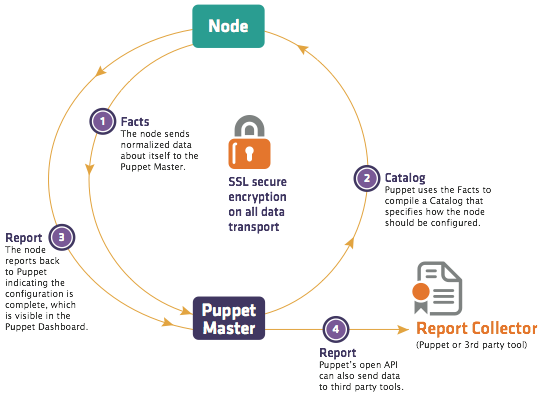
\includegraphics[width=0.8\textwidth]{images/puppet_dataflow.png}}
  \end{center}
\end{frame}

\subsubsection*{Các thành phần chính của Puppet}
\begin{frame}{Các thành phần chính của Puppet}
  \begin{itemize}
    \item \textbf{Agent}: Thực hiện những công việc mà Puppet Master yêu cầu.
    \pause
    \item \textbf{Facter}: Thu thập các thông tin cần thiết cho Puppet Master.
    \pause
    \item \textbf{External Node Classifier}\\ Các lớp mở rộng.
    \pause
    \item \textbf{Compiler} \\ Trình biên dịch các thông tin cấu hình.
  \end{itemize}
\end{frame}

\begin{frame}{Các thành phần chính của Puppet}
  \begin{itemize}
    \item \textbf{Transaction} \\ Trao đổi các Catalog giữa agent và master.
    \pause
    \item \textbf{Resource Abstraction Layer} \\ Các lớp tài nguyên trừu tượng.
    \pause
    \item \textbf{Reporting} \\ Các bản báo cáo.
  \end{itemize}
\end{frame}

\subsection{Chef}
\subsubsection*{Tổng quan về Chef}

\begin{frame}{Tổng quan về Chef}
\renewcommand{\baselinestretch}{1.50}\normalsize
  \begin{itemize}
    \item \textbf{Chef} là một phần mềm \textbf{Mã Nguồn Mở} được viết bằng Ruby.
    \pause
    \item \textbf{Chef} là một công cụ tự động hóa hệ thống và cơ sở hạ tầng điện toán đám mây.
    \pause
    \item \textbf{Chef} có khả năng triển khai các máy chủ hoặc các ứng dụng tới bất kì đâu.
  \end{itemize}
\renewcommand{\baselinestretch}{1.0}\normalsize
\end{frame}

\subsubsection*{Kiến trúc hệ thống của Chef}
\begin{frame}{Kiến trúc hệ thống của Chef}
  \begin{center}
  \fbox{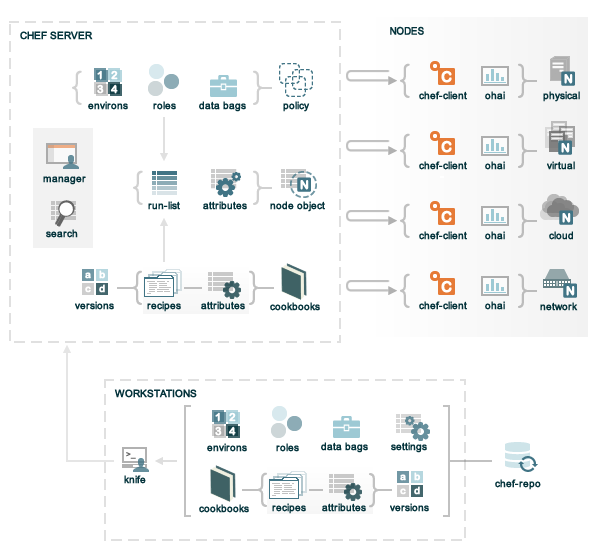
\includegraphics[width=0.65\textwidth]{images/chef_overview.png}}
  \end{center}
\end{frame}

\subsubsection*{Các thành phần chính của Chef}
\begin{frame}{Các thành phần chính của Chef}
  \begin{itemize}
    \item \textbf{Các nút}: máy chủ vật lý, máy chủ ảo, máy chủ điện toán đám mây hay thiết bị mạng.
    \pause
    \item \textbf{Máy trạm}: nơi được cấu hình để chạy Knife, nơi lưu trữ chef-repo.
    \pause
    \item \textbf{Knife}: một công cụ dòng lệnh cung cấp giao diện tương tác giữa chef-repo với máy chủ hoặc máy trạm.
  \end{itemize}
\end{frame}


\begin{frame}{Các thành phần chính của Chef}
\renewcommand{\baselinestretch}{1.50}\normalsize
  \begin{itemize}
    \item \textbf{Chef-repo}: nơi lưu trữ các đối tượng dữ liệu.
    \pause
    \item \textbf{Máy chủ}: trung tâm chứa dữ liệu cấu hình.
    \pause
    \item \textbf{Cookbook}: đơn vị cơ bản của Chef. Mỗi cookbook định nghĩa một kịch bản cấu hình.
  \end{itemize}
\renewcommand{\baselinestretch}{1.0}\normalsize
\end{frame}

\subsection{Ansible}
\subsubsection*{Tổng quan về Ansible}

\begin{frame}{Tổng quan về Ansible}
\renewcommand{\baselinestretch}{1.50}\normalsize
  \begin{itemize}
    \item \textbf{Ansible} là một công cụ tự động hóa \textbf{Mã Nguồn Mở} được viết bằng Python.
    \pause
    \item \textbf{Ansible} rất dễ học và sử dụng nhưng lại rất mạnh mẽ.
    \pause
    \item \textbf{Ansible} được thiết kế nhỏ gọn, tiện dụng, an toàn và có độ tin cậy cao.
  \end{itemize}
\renewcommand{\baselinestretch}{1.0}\normalsize
\end{frame}


\subsubsection*{Kiến trúc hệ thống của Ansible}

\begin{frame}{Kiến trúc hệ thống của Ansible}
  \begin{center}
  \fbox{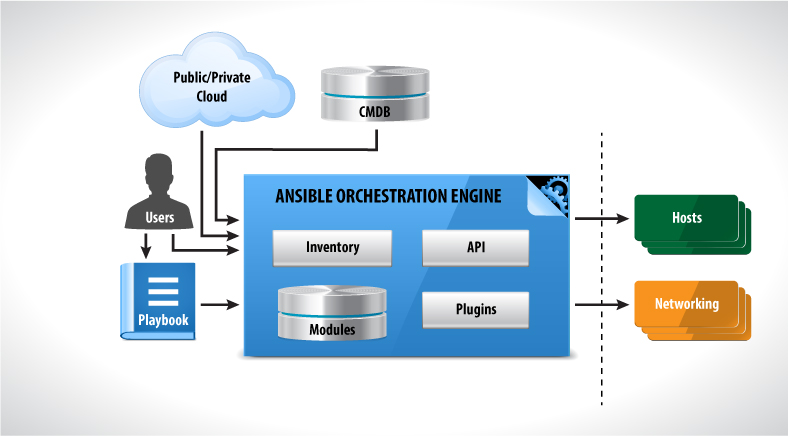
\includegraphics[width=0.8\textwidth]{images/ansible_architect.jpg}}
  \end{center}
\end{frame}


\begin{frame}{Sự khác biệt trong kiến trúc của Ansible}
\renewcommand{\baselinestretch}{1.50}\normalsize
  \begin{itemize}
    \item \textbf{Ansible} quản lý các máy trạm thông qua giao thức SSH.
    \item \textbf{Ansible} có thể sử dụng nhiều phương thức điều khiển khác nhau và có thể thay đổi được.
    \item \textbf{Ansible} không yêu cầu quyền root, nó chỉ sử dụng sudo khi cần thiết.
  \end{itemize}
\renewcommand{\baselinestretch}{1.0}\normalsize
\end{frame}


\begin{frame}{Sự khác biệt trong kiến trúc của Ansible}
\renewcommand{\baselinestretch}{1.50}\normalsize
  \begin{itemize}
    \item \textbf{Ansible} không cần một khóa SSH hay một người dùng riêng.
    \item \textbf{Ansible} sẽ chuyển các module tới nút điều khiển khi cần thiết nhưng không để lại bất cứ cài đặt gì trên nút này.
    \item \textbf{Ansible} không yêu cầu bất kì phần mềm máy chủ nào.
  \end{itemize}
\renewcommand{\baselinestretch}{1.0}\normalsize
\end{frame}

\begin{frame}{Sự khác biệt trong kiến trúc của Ansible}
  \begin{itemize}
    \item \textbf{Ansible} không yêu cầu phải có agent trên các nút điều khiển.
    \item \textbf{Ansible} không cần cấu hình phức tạp về hạ tầng mạng hay PKI.
    \item \textbf{Ansible} không chiếm tài nguyên của nút điều khiển.
  \end{itemize}
\renewcommand{\baselinestretch}{1.0}\normalsize
\end{frame}

\subsubsection*{Các thành phần chính của Ansible}

\begin{frame}{Các thành phần chính của Ansible}
\renewcommand{\baselinestretch}{1.20}\normalsize
\begin{itemize}
\item \textbf{Modules}: Ansible có rất sẵn các module phục vụ hầu hết các công việc cơ bản của ngành IT.
\pause
\item \textbf{Plugins}: Ansible có rất nhiều các thành phần để chúng ta có thể tích hợp thêm những thứ cần thiết.
\pause
\item \textbf{Playbooks}: là tập hợp những cấu hình cụ thể thực hiện một số các công việc nhất định.
\end{itemize}
\renewcommand{\baselinestretch}{1.0}\normalsize
\end{frame}

\section{Triển khai thực nghiệm}
\subsection{Bài toán}
\begin{frame}{Bài toán}
\renewcommand{\baselinestretch}{1.50}\normalsize
  \begin{alertblock}\justifying
    \emph{\textbf{"Viết công cụ tự động tạo ra một máy chủ trên nền điện toán đám mây Google Compute Engine (GCE). Sau đó tự động cài đặt và cấu hình hệ thống LAMP; cùng với đó là tự động triển khai CMS Wordpress phiên bản mới nhất lên trên máy chủ vừa tạo."}}
  \end{alertblock}
\renewcommand{\baselinestretch}{1.0}\normalsize
\end{frame}

\subsection{Phân tích}
\subsubsection*{Lựa chọn công cụ}
\begin{frame}{Lựa chọn công cụ}
\renewcommand{\baselinestretch}{1.50}\normalsize
Ansible được chọn vì những lý do sau:
\begin{itemize}
\item Ansible rất dễ học và sử dụng.
\item Ansible được viết bằng Python.
\item Ansible phù hợp với tư duy của người quản trị hệ thống.
\renewcommand{\baselinestretch}{1.0}\normalsize
\end{itemize}
\end{frame}


\begin{frame}{Phân tích}
\renewcommand{\baselinestretch}{1.50}\normalsize
Những công việc cần phải thực hiện:
\begin{itemize}
\item Tạo máy chủ ảo trên hệ thống GCE.
\item Cài đặt và cấu hình LAMP.
\item Triển khai ứng dụng Wordpress CMS.
\end{itemize}
\renewcommand{\baselinestretch}{1.0}\normalsize
\end{frame}

\subsubsection*{Tạo máy chủ ảo trên hệ thống GCE}
\begin{frame}{Tạo máy chủ ảo trên hệ thống GCE}
\begin{center}
\Large Hệ thống GCE đã được \\
Ansible hỗ trợ sẵn qua module \href{http://www.ansibleworks.com/docs/modules.html\#gce}{\textbf{\textit{gce}}}
\end{center}
\end{frame}

\subsubsection*{Cài đặt và cấu hình LAMP}
\begin{frame}{Cài đặt và cấu hình LAMP}
\begin{itemize}
\item \Large Nginx
\item \Large MySQL
\item \Large PHP
\end{itemize}
\end{frame}

\subsubsection*{Triển khai ứng dụng Wordpress CMS}
\begin{frame}{Triển khai ứng dụng Wordpress CMS}
\begin{itemize}
\item Download và giải nén mã nguồn.
\item Tạo người dùng và cơ sở dữ liệu.
\item Copy file cấu hình.
\end{itemize}
\end{frame}

\subsection{Triển khai}
\begin{frame}{Triển khai viết playbook cho Ansible}
\begin{itemize}
\item \href{run:./src/gce-wordpress-nginx/roles/gce/tasks/main.yml}{play gce}
\item \href{run:./src/gce-wordpress-nginx/roles/mysql/tasks/main.yml}{play mysql}
\item \href{run:./src/gce-wordpress-nginx/roles/nginx/tasks/main.yml}{play nginx}
\item \href{run:./src/gce-wordpress-nginx/roles/wordpress/tasks/main.yml}{play wordpress}
\end{itemize}
\end{frame}

\section{Demo}
\begin{frame}
  \begin{center}
  \fbox{
\includegraphics[width=0.7\textwidth]{images/demo.png}}
  \end{center}
\end{frame}

\section*{}
\begin{frame}
\begin{center}
\Huge Questions?
\end{center}
\end{frame}

\section*{}
\begin{frame}
    \begin{center}
        \Huge Cám ơn mọi người đã lắng nghe!
    \end{center}
\end{frame}

\end{document}
